%\begin{frame}{Opgave 8: Chebyshevpunkter}
%    Vi erstatter nu de ækvidistante punkter $x_j , j = 0, 1, \ldots , N$ med Chebyshevpunkterne $\Tilde{x}_j = 3 \frac{(1 -\cos(\frac{j \pi}{N}))}{2}, j = 0, 1, \ldots , N$. 
%    Gennemfør den grafiske undersøgelse fra punkt 4 ovenfor med dette valg af knudepunkter. 
%    Hvad kan man konkludere ud fra denne undersøgelse?
%\end{frame}

\begin{frame}{Chebyshevpunkter}
$\Tilde{x}_j = 3 \frac{(1 -\cos(\frac{j \pi}{N}))}{2}, j = 0, 1, \ldots , N$ \\
    Ved valg af Chebyshevpunkterne som $x$-værdier sker der ikke de store udsving omkring grænseværdierne, og der ses tendens til at fejlen stabiliseres omkring $10^{{-14}}$ ved $N=40$ og frem, uoverenstemmelsen mellem teoretisk og faktisk fejl skyldes her afrundingsfejl. 
    Der er dog små udsving i værdien herefter og ikke et entydigt mønster i, hvorvidt aproksimationen bliver bedre.
    At aproksimationen stabliseres omkring yderpunkterne er endvidere i overenstemmelse med teorien, hvor disse netop er karakteriseret ved at minimere Runges fænomen.
   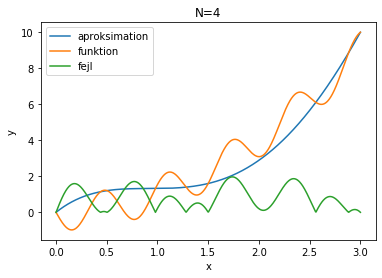
\includegraphics[scale=0.40]{images/chev_N=4.png}
   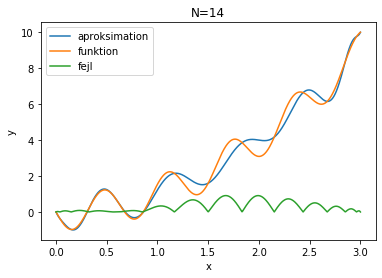
\includegraphics[scale=0.40]{images/Chev_N=14.png}
\end{frame}